\documentclass{article}
\usepackage{amsmath}
\usepackage{tikz}
\usetikzlibrary{arrows.meta}
\usetikzlibrary{decorations.pathmorphing}

\begin{document}

\begin{figure}[h]
    \centering
    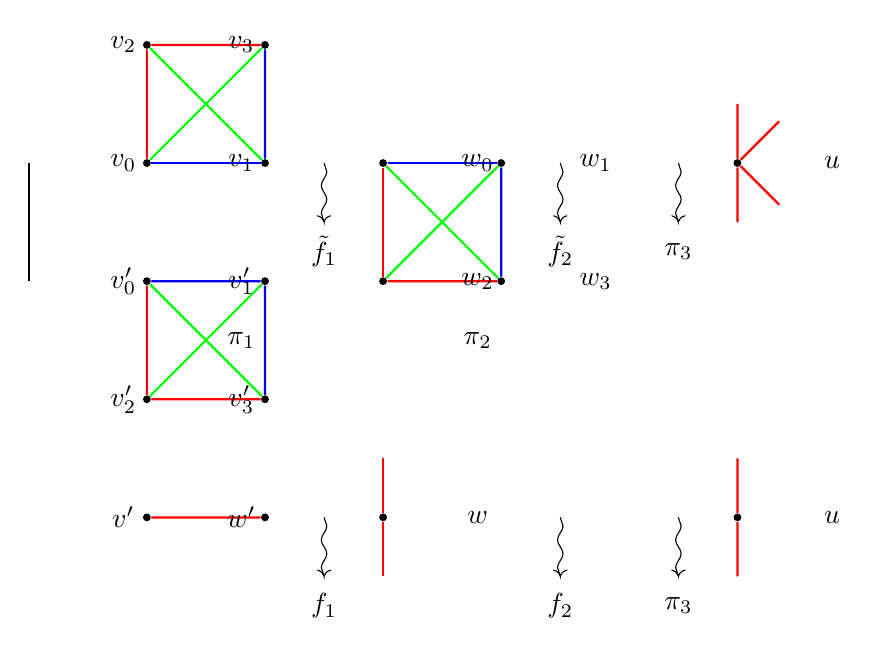
\begin{tikzpicture}[scale=1.5]
        % Nodes for the initial graph
        \node (v0) at (-2, 0) [circle, fill=black, inner sep=1pt] {};
        \node (v1) at (-1, 0) [circle, fill=black, inner sep=1pt] {};
        \node (v2) at (-2, 1) [circle, fill=black, inner sep=1pt] {};
        \node (v3) at (-1, 1) [circle, fill=black, inner sep=1pt] {};
        
        % Edges for the initial graph
        \draw[thick, blue] (v0) -- (v1);
        \draw[thick, red] (v0) -- (v2);
        \draw[thick, green] (v1) -- (v2);
        \draw[thick, blue] (v1) -- (v3);
        \draw[thick, red] (v2) -- (v3);
        \draw[thick, green] (v0) -- (v3);
        
        % Labels for the initial graph
        \node at (-2.2, 0) {$v_0$};
        \node at (-1.2, 0) {$v_1$};
        \node at (-2.2, 1) {$v_2$};
        \node at (-1.2, 1) {$v_3$};
        
        % Nodes for the first 3-cover
        \node (v0') at (-2, -1) [circle, fill=black, inner sep=1pt] {};
        \node (v1') at (-1, -1) [circle, fill=black, inner sep=1pt] {};
        \node (v2') at (-2, -2) [circle, fill=black, inner sep=1pt] {};
        \node (v3') at (-1, -2) [circle, fill=black, inner sep=1pt] {};
        
        % Edges for the first 3-cover
        \draw[thick, blue] (v0') -- (v1');
        \draw[thick, red] (v0') -- (v2');
        \draw[thick, green] (v1') -- (v2');
        \draw[thick, blue] (v1') -- (v3');
        \draw[thick, red] (v2') -- (v3');
        \draw[thick, green] (v0') -- (v3');
        
        % Labels for the first 3-cover
        \node at (-2.2, -1) {$v'_0$};
        \node at (-1.2, -1) {$v'_1$};
        \node at (-2.2, -2) {$v'_2$};
        \node at (-1.2, -2) {$v'_3$};
        
        % Arrows and labels for the first morphism
        \draw[->, decoration={snake, amplitude=1pt}, decorate] (-0.5, 0) -- (-0.5, -0.5);
        \node at (-0.5, -0.75) {$\tilde{f}_1$};
        
        % Nodes for the second 3-cover
        \node (w0) at (0, 0) [circle, fill=black, inner sep=1pt] {};
        \node (w1) at (1, 0) [circle, fill=black, inner sep=1pt] {};
        \node (w2) at (0, -1) [circle, fill=black, inner sep=1pt] {};
        \node (w3) at (1, -1) [circle, fill=black, inner sep=1pt] {};
        
        % Edges for the second 3-cover
        \draw[thick, blue] (w0) -- (w1);
        \draw[thick, red] (w0) -- (w2);
        \draw[thick, green] (w1) -- (w2);
        \draw[thick, blue] (w1) -- (w3);
        \draw[thick, red] (w2) -- (w3);
        \draw[thick, green] (w0) -- (w3);
        
        % Labels for the second 3-cover
        \node at (0.8, 0) {$w_0$};
        \node at (1.8, 0) {$w_1$};
        \node at (0.8, -1) {$w_2$};
        \node at (1.8, -1) {$w_3$};
        
        % Arrows and labels for the second morphism
        \draw[->, decoration={snake, amplitude=1pt}, decorate] (1.5, 0) -- (1.5, -0.5);
        \node at (1.5, -0.75) {$\tilde{f}_2$};
        
        % Nodes for the third 3-cover
        \node (u) at (3, 0) [circle, fill=black, inner sep=1pt] {};
        
        % Edges for the third 3-cover
        \draw[thick, red] (u) -- ++(90:0.5);
        \draw[thick, red] (u) -- ++(-90:0.5);
        \draw[thick, red] (u) -- ++(45:0.5);
        \draw[thick, red] (u) -- ++(-45:0.5);
        
        % Label for the third 3-cover
        \node at (3.8, 0) {$u$};
        
        % Arrows and labels for the third morphism
        \draw[->, decoration={snake, amplitude=1pt}, decorate] (2.5, 0) -- (2.5, -0.5);
        \node at (2.5, -0.75) {$\pi_3$};
        
        % Nodes for the dilation graph
        \node (v) at (-2, -3) [circle, fill=black, inner sep=1pt] {};
        \node (w) at (-1, -3) [circle, fill=black, inner sep=1pt] {};
        
        % Edges for the dilation graph
        \draw[thick, red] (v) -- (w);
        
        % Labels for the dilation graph
        \node at (-2.2, -3) {$v'$};
        \node at (-1.2, -3) {$w'$};
        
        % Arrows and labels for the first dilation flow
        \draw[->, decoration={snake, amplitude=1pt}, decorate] (-0.5, -3) -- (-0.5, -3.5);
        \node at (-0.5, -3.75) {$f_1$};
        
        % Nodes for the second dilation graph
        \node (w) at (0, -3) [circle, fill=black, inner sep=1pt] {};
        
        % Edges for the second dilation graph
        \draw[thick, red] (w) -- ++(90:0.5);
        \draw[thick, red] (w) -- ++(-90:0.5);
        
        % Label for the second dilation graph
        \node at (0.8, -3) {$w$};
        
        % Arrows and labels for the second dilation flow
        \draw[->, decoration={snake, amplitude=1pt}, decorate] (1.5, -3) -- (1.5, -3.5);
        \node at (1.5, -3.75) {$f_2$};
        
        % Nodes for the third dilation graph
        \node (u) at (3, -3) [circle, fill=black, inner sep=1pt] {};
        
        % Edges for the third dilation graph
        \draw[thick, red] (u) -- ++(90:0.5);
        \draw[thick, red] (u) -- ++(-90:0.5);
        
        % Label for the third dilation graph
        \node at (3.8, -3) {$u$};
        
        % Arrows and labels for the third dilation flow
        \draw[->, decoration={snake, amplitude=1pt}, decorate] (2.5, -3) -- (2.5, -3.5);
        \node at (2.5, -3.75) {$\pi_3$};
        
        % Labels for the projection maps
        \node at (-1.2, -1.5) {$\pi_1$};
        \node at (0.8, -1.5) {$\pi_2$};
        
        % Line for the initial graph
        \draw[thick] (-3, 0) -- (-3, -1);
        
    \end{tikzpicture}
    \caption{A sequence of morphisms of $\mathbb{Z}/3$-covers corresponding to first contracting the green edge in the target graph, and then the blue edge. The dilation graph is empty in the first two $3$-covers and it is a single vertex in the third picture, so there are no dilation flows.}
    \label{fig:sequence_of_morphisms}
\end{figure}

\end{document}